\documentclass[12pt]{article}

% Specify how big is going to be the paper margins.
\usepackage[a4paper, margin=1in]{geometry}

% amsmath: Add useful commans like aligh and gather.
% amsfonts: Add useful fonts like \mathbb{R}.
% amssymb: Add useful symbles like \therefore (needs amsfonts to work).
\usepackage{amsmath, amsfonts, amssymb}

% Makes the use of colors possible.
\usepackage{xcolor}

\definecolor{color1}{HTML}{0e4a7a}
\definecolor{color2}{HTML}{1282d6}
\definecolor{color3}{HTML}{7ac1ff}

% Add Latin Modern Fonts like Sans-serif and Roman.
\usepackage{lmodern}

% Makes header and footer configurable.
\usepackage{fancyhdr}

% Makes the use of colored and configured tables possible
\usepackage[most]{tcolorbox}

% Add commands to specify theorems like \newtheorem{x}{y}.
\usepackage{amsthm}

% Enables enumeration of items.
\usepackage{enumitem}

% Enables adding images.
\usepackage{graphicx}

% Enables cool hyper references.
\usepackage[colorlinks=true, linkcolor=color2, urlcolor=color2, citecolor=color2]{hyperref}

\title{\sffamily\bfseries{Soluções Jacob Palis 2023 N2}}
\author{Samuel de Araújo Brandão}
\date{4 de Setembro de 2025}

\pagestyle{fancy}
\fancyhf{}

\fancyhead[L]{\sffamily\bfseries{Soluções Jacob Palis 2023 N2}}
\fancyhead[R]{\textcolor{color2}{Samuel Brandão}, 4 de Setembro de 2025}
\fancyfoot[C]{\thepage}
\setlength{\headheight}{14.5pt}

\tcbset{
  statementbox/.style = {
    enhanced,
    width=\textwidth,
    title={Enunciado},
    title filled,
    fonttitle=\sffamily\bfseries,
    coltitle=white,
    colbacktitle=color1,
    colback=white,
    colframe=color1,
    boxrule=1pt,
    arc=2mm,
    boxsep=2pt,
  }
}

\tcbset{
  theorembox/.style = {
    enhanced,
    width=\textwidth,
    colback=white,
    colframe=color1,
    boxrule=1pt,
    arc=2mm,
    boxsep=2pt
  }
}

\tcbset{
  lemmabox/.style = {
    enhanced,
    width=\textwidth,
    colback=white,
    colframe=color2,
    boxrule=1pt,
    arc=2mm,
    boxsep=2pt
  }
}

\renewcommand*\contentsname{\textsf{Conteúdos}}
\newcommand{\kb}[1]{\left\lfloor #1 \right\rfloor}

\begin{document}
  \maketitle
  Uma coleção de soluções para a \textbf{Jacob Palis 2023 Nível 2}, inspirada no estilo de Evan Chen.
  Pode-se encontrar todos os problemas e respostas oficiais 
  \textbf{\href{https://www.obm.org.br/content/uploads/2025/04/prova_jacob_palis_2023.pdf}{aqui}}.

  Todas as soluções foram inteiramente escritas por mim, enquanto me preparava para a
  International Mathematical Olympiad (IMO).

  Caso encontre algum erro ou tiver sugestões ou comentários, sinta-se a vontade 
  para entrar em contato!

  \tableofcontents

  \clearpage

  \section{\textsf{Problemas}}
    \subsection{Testes}
      \begin{enumerate}[label=\textbf{\arabic*.}]
        \item Ana foi à feira com 20 reais, comprou 3 bananas e 2 peras e recebeu certo valor de troco. Mais tarde, seu irmão João foi ao
          mesmo local com 29 reais, comprou 5 bananas e 3 peras e também recebeu troco. Depois Maria, mãe de João e Ana, comprou mais uma
          banana e uma pera. Sabendo que Ana, João e Maria receberam a mesma quantia de troco, quantos reais Maria levou para a feira?
        \item Regis vai comprar uma capinha personalizada de celular na internet. A capinha custa 100 reais, o frete custa 20 reais e a
          personalização custa 30 reais. Regis possui dois cupons de desconto, mas só pode usar um deles. O primeiro dá frete grátis e o
          segundo dá desconto de 20\% no total da compra (capinha, frete e personalização). Se Regis usar o cupom no qual paga o menor valor
          possível, quanto Regis vai pagar?
        \item José preencheu um tabuleiro $3\times3$ com os números de 1 a 9 e notou que a soma dos números em \(k\) filas (linhas ou colunas)
          era ímpar. Quantos são os possíveis valores para \(k\)?
        \item Qual é o número mínimo de cores necessárias para colorir as bolinhas da figura abaixo de modo que bolinhas ligadas por um
          segmento tenham cores distintas?
          \begin{figure}[h]
            \centering
            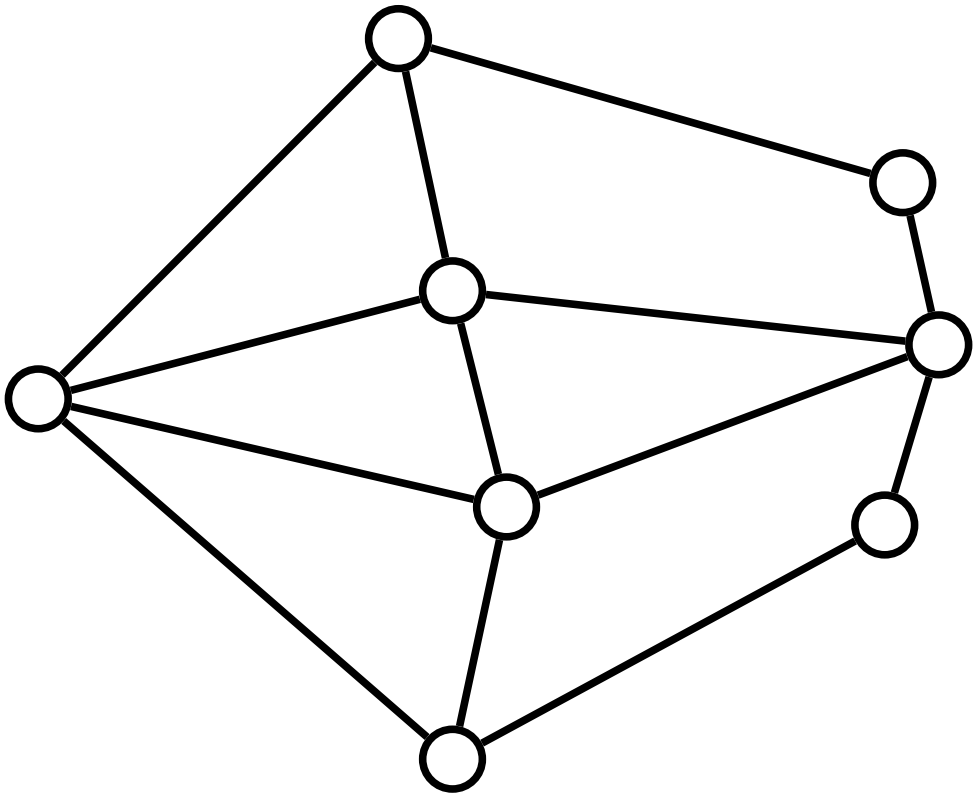
\includegraphics[width=0.3\textwidth]{first.png}
          \end{figure}
        \item José escreveu no quadro a igualdade
          \[
            2^n + 2^n + \cdots + 2^n = 15360.
          \]
          Maria percebeu que havia \(2m+1\) parcelas iguais a \(2^n\) no lado esquerdo, sendo \(m\) um número inteiro. Quanto vale \(m+n\)?
        \item O número de seis algarismos \(N = (2aaaa6)\) é divisível por 24. A soma dos algarismos de \(N\) é quanto?
        \item Sendo \(x\) e \(y\) reais tais que
          \[
            \frac{x+1^2}{y+1} = \frac{x+2^2}{y+2} = k,
          \]
          quanto vale \(k\)?
        \item De quantas maneiras podemos pintar as letras da palavra JACOB se as vogais devem ser coloridas de azul ou vermelho e as
          consoantes devem ser coloridas de azul ou verde e, além disso, não podemos ter letras adjacentes com a mesma cor?

        \item As letras \(O, B, M, J, P\) representam algarismos distintos. Sabendo que
          \[
            OBM + OBM = JP \cdot JP,
          \]
          qual é o valor de \(O+B+M+J+P\)?
        \item Na figura a seguir, \(ABCD\) é um paralelogramo. Os pontos \(M\) e \(N\) são pontos médios de \(DP\) e \(BP\), respectivamente.
          Se a área do paralelogramo \(ABCD\) é 24, qual é a área da região sombreada?
          \begin{figure}[h]
            \centering
            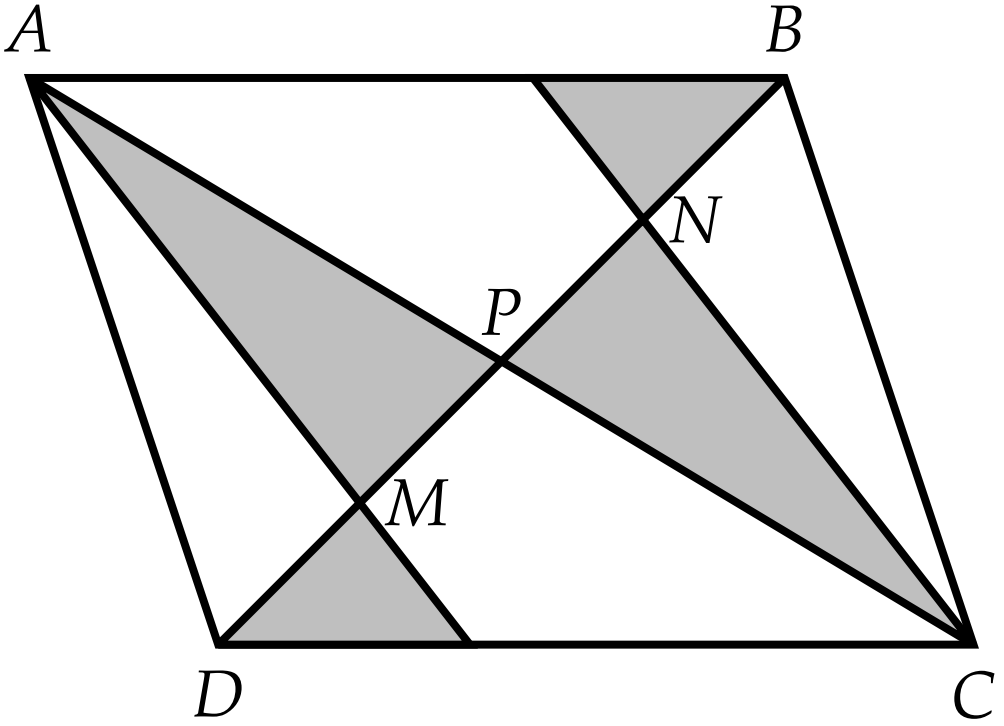
\includegraphics[width=0.3\textwidth]{second.png}
          \end{figure}
        \item Seja $X$ um subconjunto de ${1, 2, \dots,2023}$ (conjunto dos inteiros de $1$ até $2023$) tal que se $a$ e $b$ pertencem a $X$, então $a + b$
          não é múltiplo de $3$. Qual é o maior valor possível da quantidade de elementos de \(X\)?
        \item O número
          \[
            \sqrt{2022^2 + 2023^2 + (2022\cdot2023)^2} + \sqrt{2023^2 + 2024^2 + (2023\cdot2024)^2}
          \]
          é
          \begin{enumerate}[label=({\Alph*})]
            \item número irracional 
            \item inteiro e múltiplo de $3$ 
            \item inteiro e múltiplo de $5$ 
            \item inteiro e múltiplo de $8$ 
            \item primo?
          \end{enumerate}
        \item No triângulo acutângulo \(ABC\), \(AH\) é altura, com \(H\) sobre \(BC\). Sejam \(P\) e \(Q\) as projeções de \(H\) em \(AB\)
          e \(AC\), respectivamente. Sabendo que \(\angle ABC - \angle ACB = 20^\circ\). Qual é a medida do ângulo agudo determinado pelas retas \(PQ\)
          e \(AH\)?
        \item Sejam \(a\) e \(b\) números reais. As raízes da equação \(x^2 - a x + b = 0\) são \(r\) e \(s\), e as raízes da equação
          \(x^2 - (b+3)x + (a+3) = 0\) são \(\frac{1}{r}\) e \(\frac{1}{s}\). Então \((b+1)^3\) é igual a quê?
        \item Considere que \(n\) times de futebol jogam exatamente uma vez contra cada um dos outros \(n-1\) times. Em cada partida, o time 
          vencedor ganha 3 pontos e o perdedor 0; em caso de empate, cada time ganha 1 ponto. Ao fim do campeonato, ordenamos os times por 
          pontos em ordem decrescente. 

          Para \(n=3\), há sete possibilidades de pontuações dos três times: (6; 3; 0), (6; 1; 1), (4; 4; 0), (4; 3; 1), (4; 2; 1), (3; 3; 3)
          e (2; 2; 2).

          Para \(n=4\), há quantas possibilidades de pontuação dos quatro times?
      \end{enumerate}
    \subsection{Respostas Numéricas}
      \begin{enumerate}[label=\textbf{\arabic*.}, start=16]
      \item Se \(a\) e \(b\) são inteiros positivos tais que \(\operatorname{mdc}(a,b) = 6\) e \(\operatorname{mmc}(a,b) = 36a^2\), quanto vale \(a+b\)?
      \item De quantos modos podemos colorir um tabuleiro \(2\times8\) de modo que cada quadrado unitário seja verde ou amarelo e cada 
        quadrado \(2\times2\) possua três quadrados unitários de uma cor e o outro da cor oposta?
      \item No trapézio retângulo \(ABCD\), com \(\angle ABC = \angle BCD = 90^\circ\), a base \(AB\) mede 104 e a base \(CD\) mede 234.
        Sabendo que a bissetriz do ângulo \(D\) intersects \(BC\) no seu ponto médio, determine a medida do lado \(BC\).
        \begin{figure}[h]
          \centering
          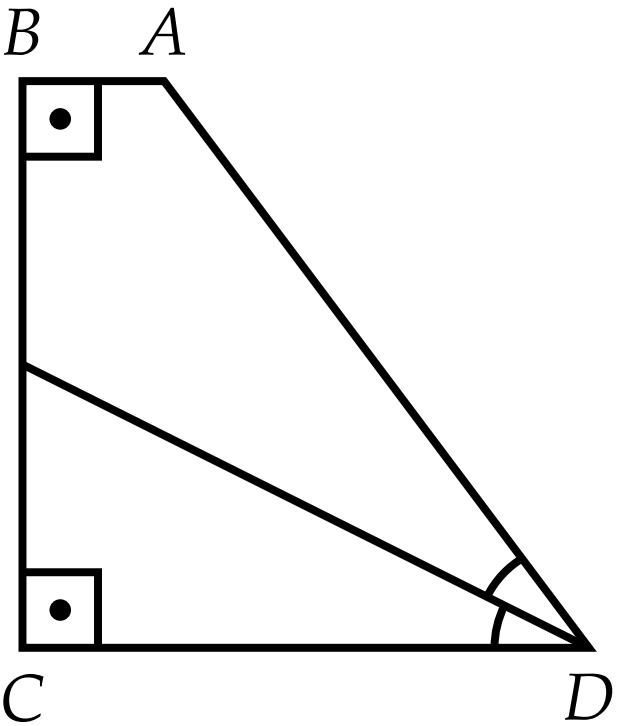
\includegraphics[width=0.25\textwidth]{third.png}
        \end{figure}
      \item Um número é chamado de perfeitoso quando nenhum dos seus algarismos é zero e a soma dos seus algarismos é um quadrado perfeito.
        Por exemplo, 97, 112 e 1111 são números perfeitosos com 2, 3 e 4 algarismos, respectivamente. Luiz escreveu todos os números 
        perfeitosos de 2023 algarismos. Quantos valores possíveis para a soma dos algarismos dos números da lista?
      \item A \textit{sequência de Fibonacci} é uma sequência em que cada termo, a partir do terceiro, é a soma dos dois termos imediatamente
        anteriores, sendo os dois termos iniciais iguais a $1$. Então, os primeiros termos da sequência são:
        \[
          1, 1, 2, 3, 5, 8, 13, 21, 34, 55, 89, \dots
        \]
        Dentre os $100$ primeiros termos da sequência, quantos são múltiplos de $3$ \textbf{ou} $4$?
    \end{enumerate}

  \clearpage

  \section{\textsf{Soluções}}
  \subsection{Problema 1}
\begin{tcolorbox}[statementbox]
Ana foi à feira com 20 reais, comprou 3 bananas e 2 peras e recebeu certo valor de troco. Mais tarde, seu irmão João foi ao
mesmo local com 29 reais, comprou 5 bananas e 3 peras e também recebeu troco. Depois Maria, mãe de João e Ana, comprou mais uma
banana e uma pera. Sabendo que Ana, João e Maria receberam a mesma quantia de troco, quantos reais Maria levou para a feira?
\end{tcolorbox}

\clearpage

\subsection{Problema 2}
\begin{tcolorbox}[statementbox]
Regis vai comprar uma capinha personalizada de celular na internet. A capinha custa 100 reais, o frete custa 20 reais e a
personalização custa 30 reais. Regis possui dois cupons de desconto, mas só pode usar um deles. O primeiro dá frete grátis e o
segundo dá desconto de 20\% no total da compra (capinha, frete e personalização). Se Regis usar o cupom no qual paga o menor valor
possível, quanto Regis vai pagar?
\end{tcolorbox}

\clearpage

\subsection{Problema 3}
\begin{tcolorbox}[statementbox]
José preencheu um tabuleiro \(3\times3\) com os números de 1 a 9 e notou que a soma dos números em \(k\) filas (linhas ou colunas)
era ímpar. Quantos são os possíveis valores para \(k\)?
\end{tcolorbox}

\clearpage

\subsection{Problema 4}
\begin{tcolorbox}[statementbox]
Qual é o número mínimo de cores necessárias para colorir as bolinhas da figura abaixo de modo que bolinhas ligadas por um
segmento tenham cores distintas?
\begin{center}
  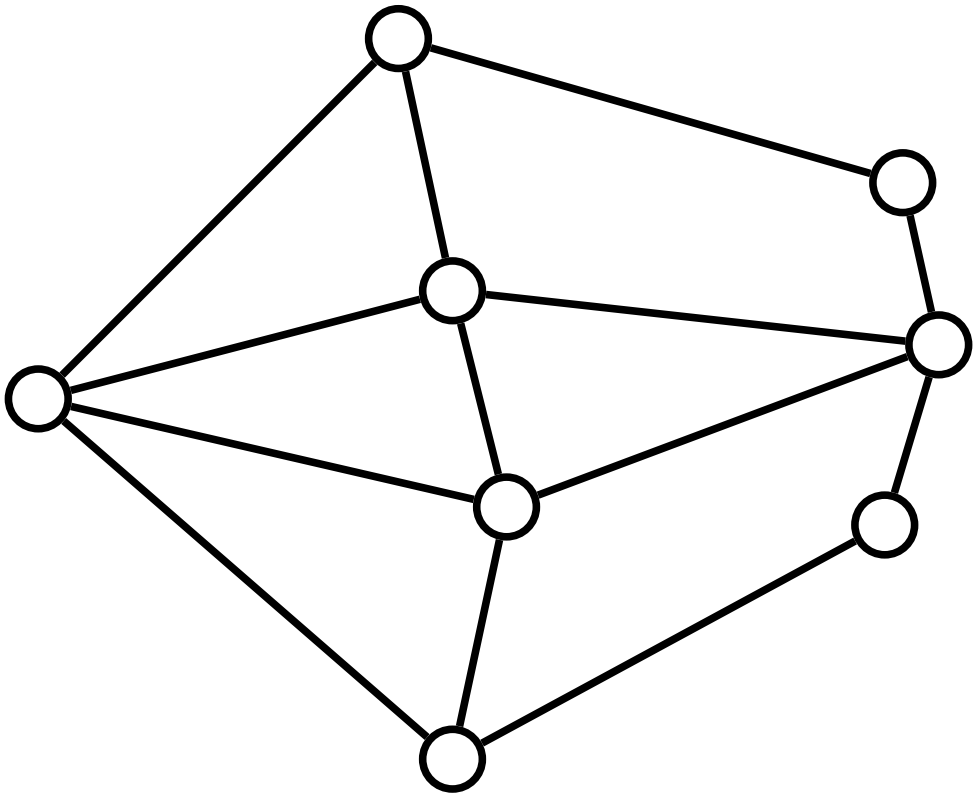
\includegraphics[width=0.25\textwidth]{first.png}
\end{center}
\end{tcolorbox}

\clearpage

\subsection{Problema 5}
\begin{tcolorbox}[statementbox]
José escreveu no quadro a igualdade
\[
  2^n + 2^n + \cdots + 2^n = 15360.
\]
Maria percebeu que havia \(2m+1\) parcelas iguais a \(2^n\) no lado esquerdo, sendo \(m\) um número inteiro. Quanto vale \(m+n\)?
\end{tcolorbox}

\clearpage

\subsection{Problema 6}
\begin{tcolorbox}[statementbox]
O número de seis algarismos \(N = (2aaaa6)\) é divisível por 24. A soma dos algarismos de \(N\) é quanto?
\end{tcolorbox}

\clearpage

\subsection{Problema 7}
\begin{tcolorbox}[statementbox]
Sendo \(x\) e \(y\) reais tais que
\[
  \frac{x+1^2}{y + 1} = \frac{x+2^2}{y+2} = k,
\]
quanto vale \(k\)?
\end{tcolorbox}

\clearpage

\subsection{Problema 8}
\begin{tcolorbox}[statementbox]
De quantas maneiras podemos pintar as letras da palavra JACOB se as vogais devem ser coloridas de azul ou vermelho e as
consoantes devem ser coloridas de azul ou verde e, além disso, não podemos ter letras adjacentes com a mesma cor?
\end{tcolorbox}

\clearpage

\subsection{Problema 9}
\begin{tcolorbox}[statementbox]
As letras \(O, B, M, J, P\) representam algarismos distintos. Sabendo que
\[
  OBM + OBM = JP \cdot JP,
\]
qual é o valor de \(O+B+M+J+P\)?
\end{tcolorbox}

\clearpage

\subsection{Problema 10}
\begin{tcolorbox}[statementbox]
Na figura a seguir, \(ABCD\) é um paralelogramo. Os pontos \(M\) e \(N\) são pontos médios de \(DP\) e \(BP\), respectivamente.
Se a área do paralelogramo \(ABCD\) é 24, qual é a área da região sombreada?
\begin{center}
  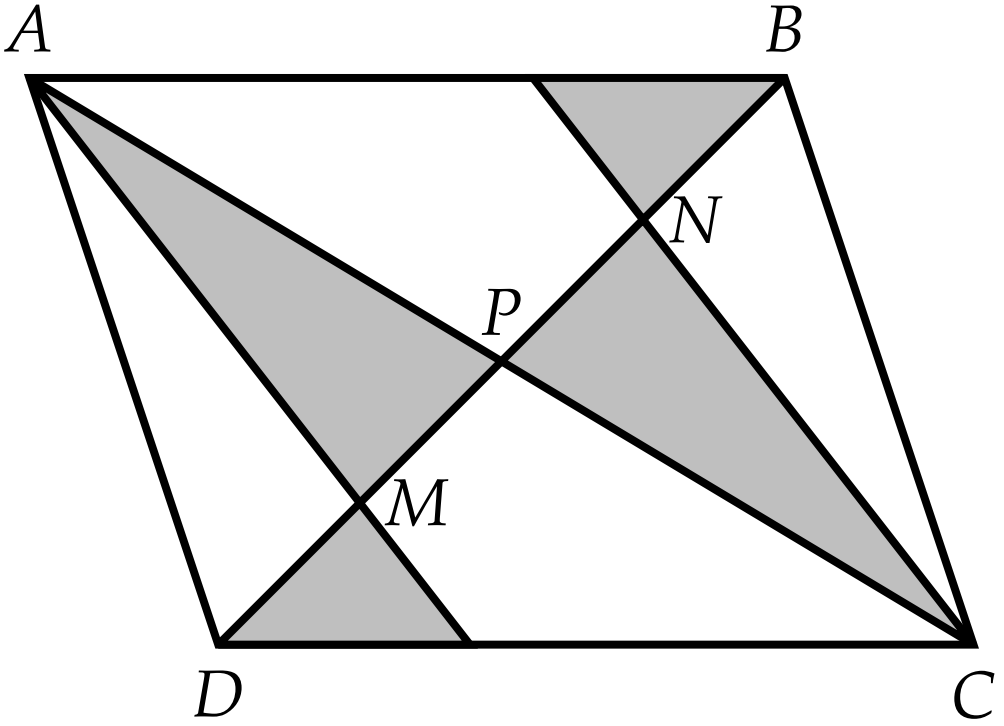
\includegraphics[width=0.25\textwidth]{second.png}
\end{center}
\end{tcolorbox}

\clearpage

\subsection{Problema 11}
\begin{tcolorbox}[statementbox]
  Seja $X$ um subconjunto de ${1, 2, \dots,2023}$ (conjunto dos inteiros de $1$ até $2023$) tal que se $a$ e $b$ pertencem a $X$, então $a + b$ 
  não é múltiplo de $3$. Qual é o maior valor possível da quantidade de elementos de \(X\)?
\end{tcolorbox}

\clearpage

\subsection{Problema 12}
\begin{tcolorbox}[statementbox]
O número
\[
  \sqrt{2022^2 + 2023^2 + (2022\cdot2023)^2} + \sqrt{2023^2 + 2024^2 + (2023\cdot2024)^2}
\]
é
\begin{enumerate}[label=({\Alph*})]
  \item número irracional 
  \item inteiro e múltiplo de $3$ 
  \item inteiro e múltiplo de $5$ 
  \item inteiro e múltiplo de $8$ 
  \item primo?
\end{enumerate}
\end{tcolorbox}

\clearpage

\subsection{Problema 13}
\begin{tcolorbox}[statementbox]
No triângulo acutângulo \(ABC\), \(AH\) é altura, com \(H\) sobre \(BC\). Sejam \(P\) e \(Q\) as projeções de \(H\) em \(AB\)
e \(AC\), respectivamente. Sabendo que \(\angle ABC - \angle ACB = 20^\circ\). Qual é a medida do ângulo agudo determinado pelas retas \(PQ\)
e \(AH\)?
\end{tcolorbox}

\clearpage

\subsection{Problema 14}
\begin{tcolorbox}[statementbox]
Sejam \(a\) e \(b\) números reais. As raízes da equação \(x^2 - a x + b = 0\) são \(r\) e \(s\), e as raízes da equação
\(x^2 - (b+3)x + (a+3) = 0\) são \(\frac{1}{r}\) e \(\frac{1}{s}\). Então \((b+1)^3\) é igual a quê?
\end{tcolorbox}

\clearpage

\subsection{Problema 15}
\begin{tcolorbox}[statementbox]
Considere que \(n\) times de futebol jogam exatamente uma vez contra cada um dos outros \(n-1\) times. Em cada partida, o time 
vencedor ganha 3 pontos e o perdedor 0; em caso de empate, cada time ganha 1 ponto. Ao fim do campeonato, ordenamos os times por 
pontos em ordem decrescente.

Para \(n=3\), há sete possibilidades de pontuações dos três times: (6; 3; 0), (6; 1; 1), (4; 4; 0), (4; 3; 1), (4; 2; 1),
(3; 3; 3) e (2; 2; 2).

Para \(n=4\), há quantas possibilidades de pontuação dos quatro times?

\end{tcolorbox}

\clearpage

\subsection{Problema 16}
\begin{tcolorbox}[statementbox]
  Se \(a\) e \(b\) são inteiros positivos tais que \(\operatorname{mdc}(a,b) = 6\) e \(\operatorname{mmc}(a,b) = 36a^2\), quanto vale \(a+b\)?
\end{tcolorbox}

\clearpage

\subsection{Problema 17}
\begin{tcolorbox}[statementbox]
De quantos modos podemos colorir um tabuleiro \(2\times8\) de modo que cada quadrado unitário seja verde ou amarelo e cada 
quadrado \(2\times2\) possua três quadrados unitários de uma cor e o outro da cor oposta?
\end{tcolorbox}

\clearpage

\subsection{Problema 18}
\begin{tcolorbox}[statementbox]
No trapézio retângulo \(ABCD\), com \(\angle ABC = \angle BCD = 90^\circ\), a base \(AB\) mede 104 e a base \(CD\) mede 234.
Sabendo que a bissetriz do ângulo \(D\) intersects \(BC\) no seu ponto médio, determine a medida do lado \(BC\).
\begin{center}
  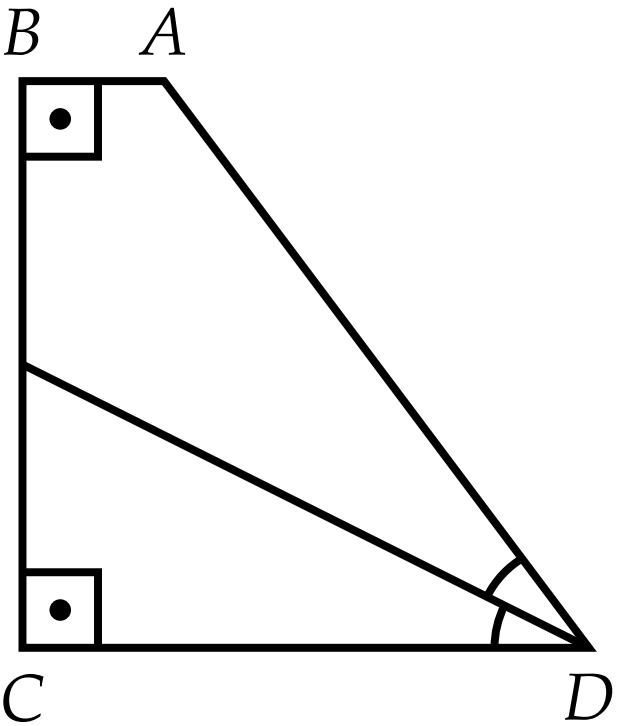
\includegraphics[width=0.25\textwidth]{third.png}
\end{center}
\end{tcolorbox}

\clearpage

\subsection{Problema 19}
\begin{tcolorbox}[statementbox]
Um número é chamado de perfeitoso quando nenhum dos seus algarismos é zero e a soma dos seus algarismos é um quadrado perfeito.
Por exemplo, 97, 112 e 1111 são números perfeitosos com 2, 3 e 4 algarismos, respectivamente. Luiz escreveu todos os números 
perfeitosos de 2023 algarismos. Quantos valores possíveis para a soma dos algarismos dos números da lista?
\end{tcolorbox}

\clearpage

\subsection{Problema 20}
\begin{tcolorbox}[statementbox]
  A \textit{sequência de Fibonacci} é uma sequência em que cada termo, a partir do terceiro, é a soma dos dois termos imediatamente
  anteriores, sendo os dois termos iniciais iguais a $1$. Então, os primeiros termos da sequência são:
  \[
    1, 1, 2, 3, 5, 8, 13, 21, 34, 55, 89, \dots
  \]
  Dentre os $100$ primeiros termos da sequência, quantos são múltiplos de $3$ \textbf{ou} $4$?
\end{tcolorbox}

  \clearpage

  \section{\textsf{Referências}}
\end{document}
